\section{Timing Diagram}
Um zeitliche Abläufe besser zu verdeutlichen, werden die Anforderungen aus den Requirements \textbf{Connection.02} und \textbf{Notification.02} mittels Timing Diagrams modelliert. Durch das Requirement \textbf{Connection.02} wird definiert, dass der Verbindungsaufbau zwischen Smartwatch und Smartphone in maximal 4 Sekunden dauern darf. Das entsprechende Timing Diagram ist in Abbildung~\ref{fig:timing_diagram_pairing} abgebildet. Dieses Diagramm enthält auch das in Phase 3 hinzugefügte \textit{Satisfy-Callout} um die Abhändigkeit mit Requirement \textbf{Connection.02} zu verdeutlichen.

\begin{figure}[H]
\centering\
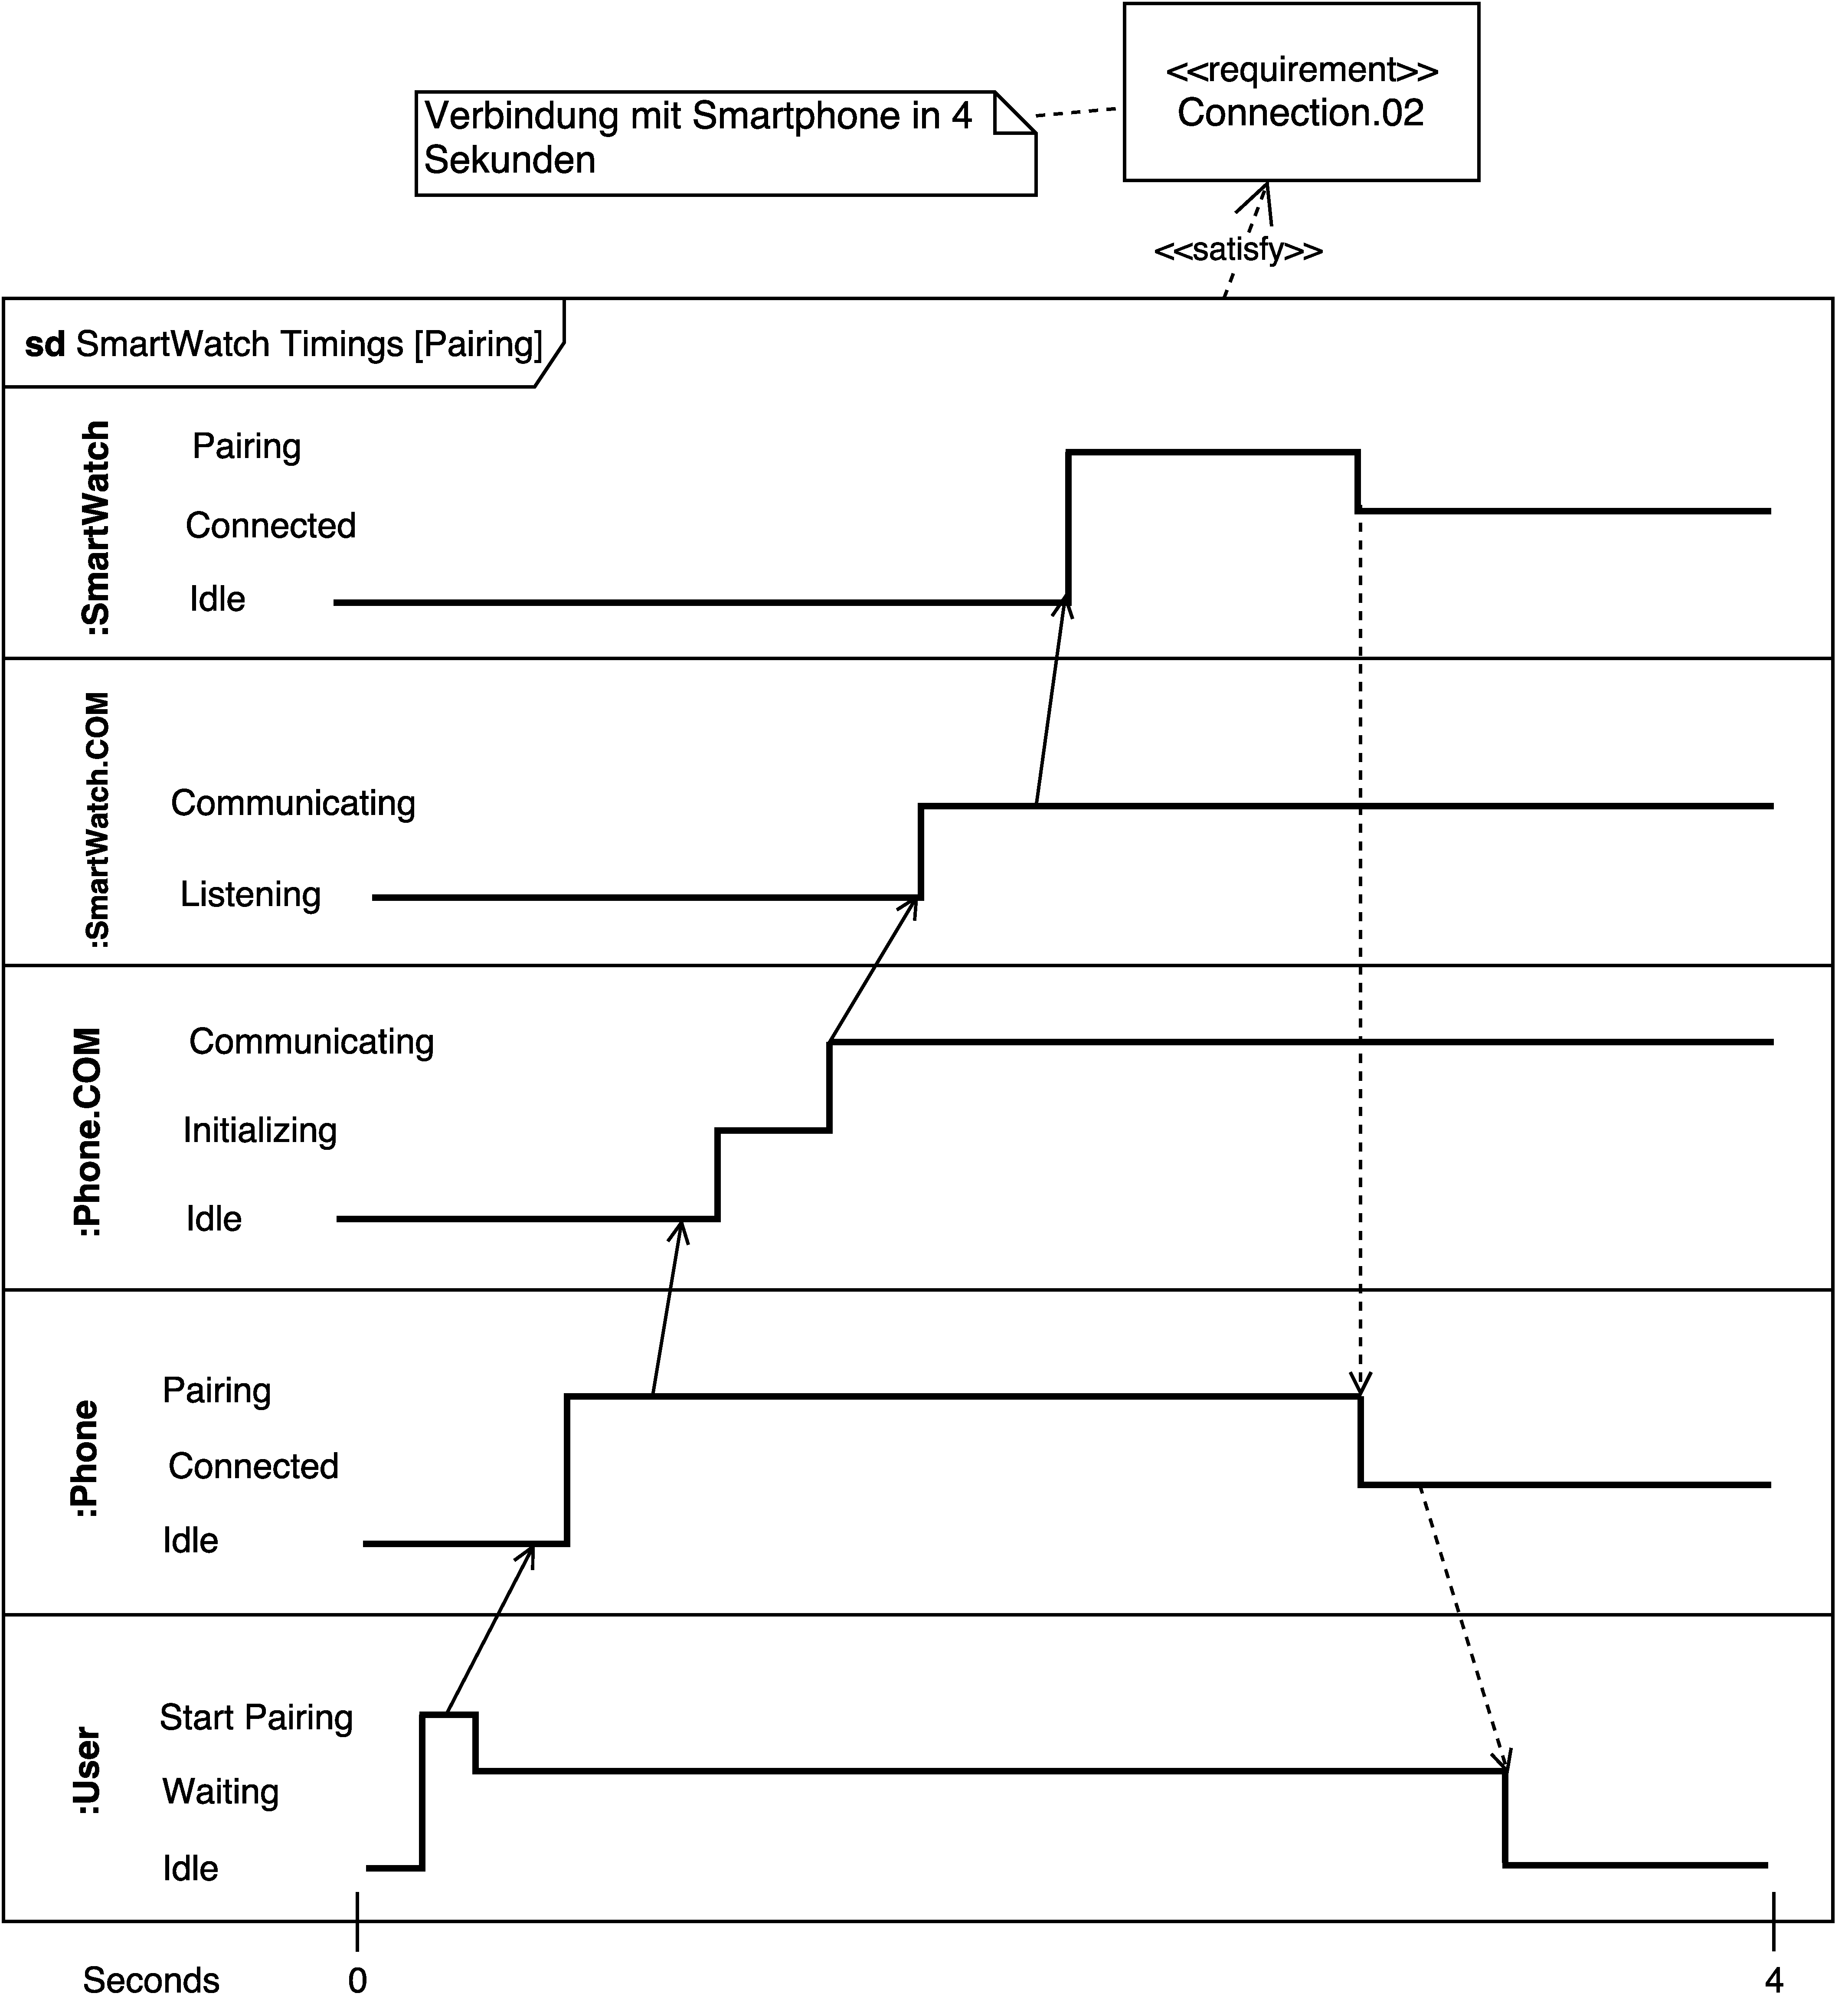
\includegraphics[width=12cm]{img/timing_diagram_pairing}
\caption[Timing Diagram: Pairing]{Modellierung der Anforderungen aus Requierement \textbf{Connection.02} als Timing Diagram. }
\label{fig:timing_diagram_pairing}
\end{figure}

Die Zeit bis zum Anzeigen einer \gls{Notification} wird im Requirement \textbf{Notification.02} detaiiliert beschrieben. Aus dem Requirement folgt, dass Notifications innerhalb einer Sekunde auf der Smartwatch angezeigt werden müssen. Dieses Verhalten ist in Abildung~\ref{fig:timing_diagram_notifications} dargestellt.

\begin{figure}[H]
\centering\
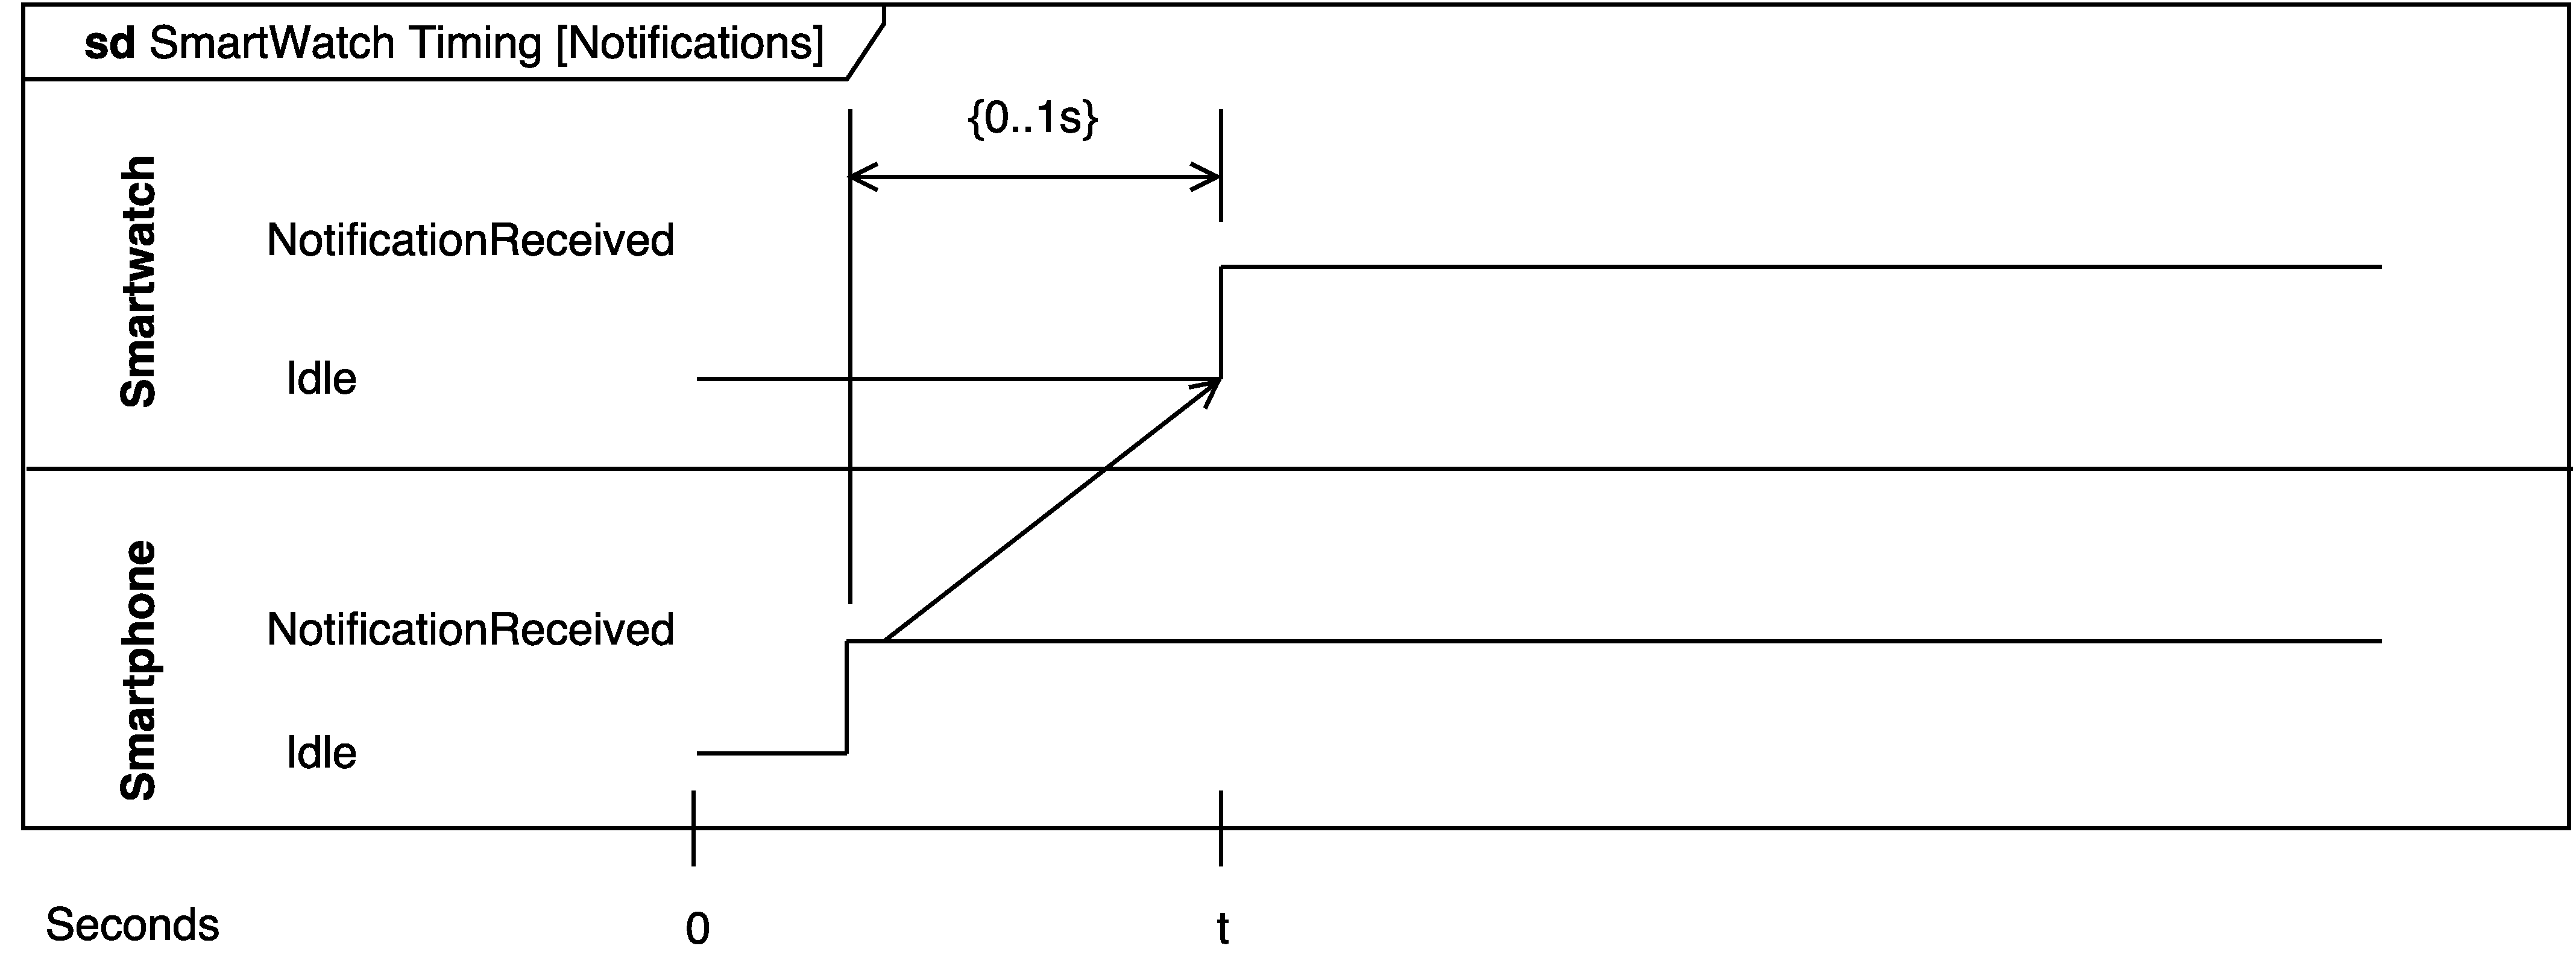
\includegraphics[width=14cm]{img/timing_diagram_notifications}
\caption[Timing Diagram: Notifications]{Modellierung der Anforderungen aus Requirement \textbf{Notification.02} bezüglich der Anzeige von Notifications als Timing Diagram.}
\label{fig:timing_diagram_pairing}
\end{figure}
